% Set the overall layout of the tree
\tikzstyle{level 1}=[level distance=3.5cm, sibling distance=3.5cm]
\tikzstyle{level 2}=[level distance=3.5cm, sibling distance=2cm]

% Define styles for bags and leafs
\tikzstyle{bag} = [text width=4em, text centered]
\tikzstyle{end} = [circle, minimum width=3pt,fill, inner sep=0pt]
\scalebox{0.75}{
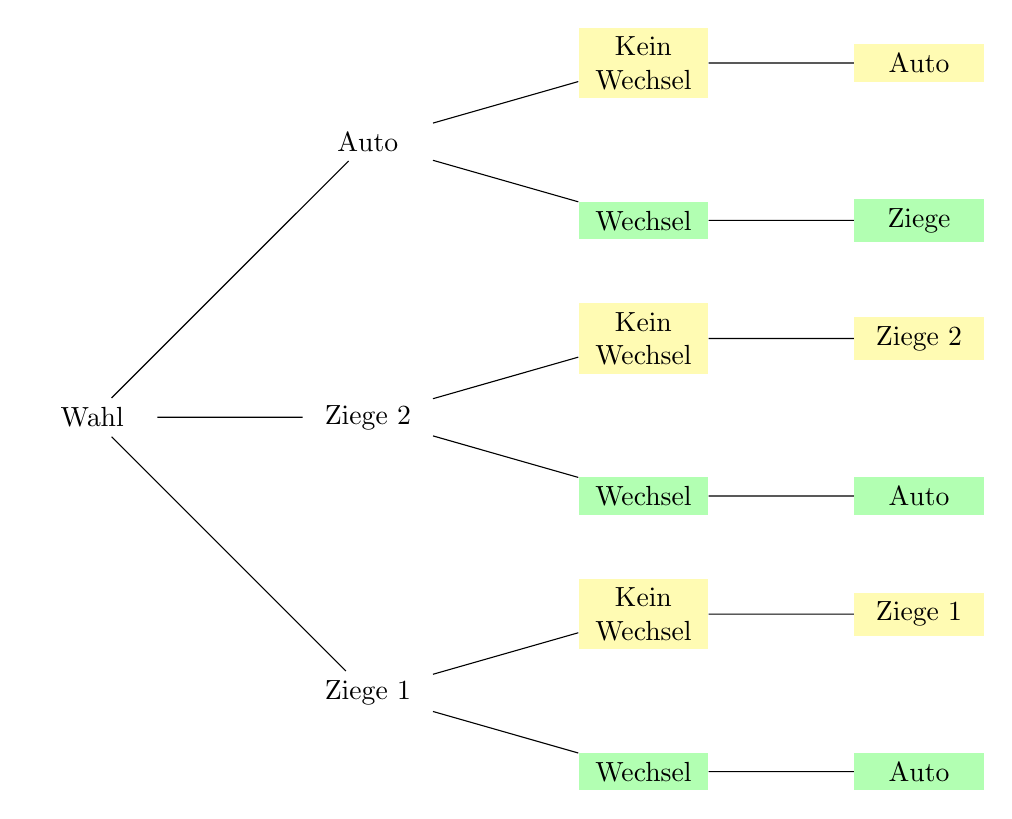
\begin{tikzpicture}[grow=right, sloped]
\node[bag] {Wahl}
    child {
        node[bag] {Ziege 1}% This is the first of three "Bag 2"
        child {
                node[bag,fill=green!30!] {Wechsel}
                child {
                    node[bag,fill=green!30!] {Auto}
                }
            }
            child {
                node[bag,fill=yellow!30!] {Kein Wechsel}
                child{
                    node[bag,fill=yellow!30!] {Ziege 1}
                }
            }
    }
    child {
        node[bag] {Ziege 2}% This is the first of three "Bag 2"
        child {
                node[bag,fill=green!30!] {Wechsel}
                child {
                    node[bag,fill=green!30!] {Auto}
                }
            }
            child {
                node[bag,fill=yellow!30!] {Kein Wechsel}
                child{
                    node[bag,fill=yellow!30!] {Ziege 2}
                }
            }
    }
        child {
            node[bag] {Auto}
            child {
                    node[bag,fill=green!30!] {Wechsel}
                    child {
                        node[bag,fill=green!30!] {Ziege}
                    }
                }
                child {
                    node[bag,fill=yellow!30!] {Kein Wechsel}
                    child{
                        node[bag,fill=yellow!30!] {Auto}
                    }
                }
    };
\end{tikzpicture}
}
